\documentclass{report}

% other packages %
%\usepackage{graphicx}
%\usepackage{titlesec}
%\usepackage{url}
\usepackage{fancybox}

% lang : french %
\usepackage[utf8]{inputenc}
\usepackage{xspace}
\usepackage[T1]{fontenc}
\usepackage[english,frenchb]{babel}
\usepackage[francais]{minitoc}
\usepackage{algorithm}
\usepackage{algorithmic}
\usepackage{graphicx}
%\usepackage[unicode,hidelinks]{hyperref}
\setcounter{minitocdepth}{1}
% mise en page %
\pagestyle{empty}
\begin{document}
\dominitoc
%%%%%%%%%%%%%%

%\documentclass[pdftex,12pt,a4paper]{report}
%\usepackage[pdftex]{graphicx}
%\usepackage[francais]{babel}
%\usepackage[utf8]{inputenc}
%\usepackage[T1]{fontenc}
%\usepackage[top=2cm, bottom=2cm, left=3cm, right=3cm]{geometry}
%\usepackage{graphicx}
%\usepackage[toc,page]{appendix}
%\usepackage{pdfpages}
%\usepackage{color}
%\usepackage{chngpage}
%\usepackage{fancyhdr}
%\usepackage[Sonny]{fncychap}
%\usepackage{titlesec, blindtext, color}
%\usepackage{lastpage}

%\setcounter{tocdepth}{3}
%\setcounter{secnumdepth}{3}
%\setlength{\headheight}{14pt}
%\renewcommand\headrulewidth{1pt}
%\fancyhead[L]{Signature}
%\fancyhead[R]{EPITA}
%\definecolor{gray75}{gray}{0.75}
%\newcommand{\hsp}{\hspace{20pt}}

%\titleformat{\chapter}[hang]{\Huge\bfseries}{\thechapter\hsp\textcolor{gray75}{|}\hsp}{0pt}{\Huge\bfseries}

%\renewcommand\footrulewidth{1pt}
%\fancyfoot[L]{Signature}
%\fancyfoot[R]{Page \thepage/\pageref{LastPage}}

%\newcommand{\HRule}{\rule{\linewidth}{0.5mm}}

%\pagestyle{fancy}

%\title{MetaHeuristique}
%\author{Thibault \textsc{Lapassade} - Fabrice \textsc{Rougeau}}
%\maketitle

\begin{titlepage}
\begin{center}
\textsc{\LARGE MetaHeuristique}\\[1.5cm]
\end{center}

\begin{minipage}{0.4\textwidth}
	\begin{flushleft} \large
		\emph{Auteurs:}\\
			Thibault \textsc{Lapassade} \\
			Fabrice \textsc{Rougeau} \\
	\end{flushleft}
\end{minipage}
\begin{minipage}{0.4\textwidth}
	\begin{flushright} \large
		\emph{Relecture:} \\
              Patrick \textsc{Siarry}
	\end{flushright}
\end{minipage}
\end{titlepage}

\tableofcontents

\chapter{Introduction}
\minitoc
Lors du cours de tronc commun nous avons étudié une métaheuristique pour l'optimisation difficile.

Suite à ce cour, nous devons mettre en pratique deux méthodes dans le cadre d'exercices pratiques, l'un traitant le cas discret avec la méthode du recuit simulé et l'autre le cas continu avec le recuit simulé ou le cas discret avec une autre métaheuristique. Ce rapport fait donc office de compte rendu du travail qui a été effectué dans cette perspective.

Pour chacun des exercices nous ferons un bref rappel du sujet, nous présenterons brièvement la méthode utilisée, nous exposerons ce qui a été réalisé et comment. Nous traiterons enfin de l'analyse des résultats et des méthodes permettant de fixes les paramètres de ces algorithmes.
\newpage

\chapter{Cas discret avec le recuit simulé}
\minitoc
\section{Rappel du sujet}
Nous allons tout d’abord rappelé le sujet de l’exercice à résoudre, en ce qui concerne
le cas discret.

Il s’agissait de résoudre un problème de placement de composants électroniques
en des sites prédéterminés. Il faut placer 25 blocs. Le seul mouvement autorisé est
la permutation de deux blocs. La fonction objectif, qu’il convient de minimiser, est
évaluée en sommant les longueurs en L (dites aussi « longueurs de Manhattan ») des
connexions. La distance entre deux blocs est égale à 5. Nous savons que pour les
configurations optimales, la fonction objectif est égale à 200, ce qui nous permettra
d’évaluer l’efficacité de notre méthode. Notons que les composants voisins sont définis dès le départ. Ainsi le composant numéro 8 doit être relié avec les composants
numéro 13, 3, 7 et 9. Les captures d’écran de notre application sont, à ce sujet, sans
doute plus claires qu’un long discours ; le lecteur perdu est donc invité à s’y référer.

Nous avons choisi d’implémenter la méthode du recuit simulé qui semblait bien
adaptée pour résoudre ce problème.

\section{Le recuit simulé}
Nous n’allons pas détailler tous les aspects de cette méthode, car ce n’est pas le
propos de ce rapport. Nous allons, toutefois, récapituler très brièvement, les grands
traits caractéristiques du recuit simulé.

Cette méthode est inspirée de la physique. L’idée vient du fait que la nature parvient à passer d’un état désordonné à un état ordonné, d’énergie globale minimum.
Le forgeron travaille en utilisant des paliers de température. La méthode utilise une
règle d’acceptation qui est souvent la règle de Métropolis.

L'idée est de partir d'un état quelconque en fixant une température T assez élevée. On perturbe cet état par une légère transformation, ce qui entraîne une variation $\Delta{E}$ du système. Si $\Delta{E} \leq 0$, on accepte le nouvel état (qui est meilleur), sinon on l'accepte avec une probabilité $\exp^{\frac{-\Delta E}{T}}$. Ce procédé permet de ne pas rester pris dans un minimum local, puisque en effet, on peut accepter des configurations dégradantes dans certaines conditions. Si l'équilibre thermodynamique est atteint, on baisse la température suivant un coefficient que l'on choisit nous même (dans notre cas, T= 0.9*T). On remarque donc que plus l'algorithme évolue, plus la température baisse et donc moins on aura tendance à accepter de configurations dégradantes. Ceci permettra de tendre vers une stabilisation dans un optimum global.
\begin{algorithm}
\caption{Algorithme du recuit simulé}
\begin{algorithmic}
\REQUIRE Configuration initiale quelconque, $\tau 0$
\ENSURE Meilleur configuration
\STATE Calcul de T à partir de $\tau 0$
\WHILE{Le système n'est pas figé}
\STATE Modification élémentaire du système qui entraine une variation $\Delta E$ du système
\IF{$\Delta E \leq 0$}
\STATE Modification acceptée
\ELSE
\STATE Modification acceptée avec la probabilité $\exp^{\frac{-\Delta E}{T}}$
\ENDIF
\IF {Equilibre thermodynamique}
\STATE Diminution lente de T
\ENDIF
\ENDWHILE
\end{algorithmic}

\end{algorithm}
\begin{algorithm}
\caption{Calcul de T à partir de $\tau 0$}
\begin{algorithmic}
\REQUIRE $\tau 0$
\ENSURE T
\STATE T = 0
\WHILE{Moins de 100 modification élémentaire}
\STATE Fait une modification élémentaire
\STATE T = T + |$\Delta E$|
\ENDWHILE
\STATE T = $T \div 100$
\STATE T = $\frac{-T}{\log \tau 0}$
\end{algorithmic}
\end{algorithm}

Voyons comment cela se traduit concrètement, en pratique, sur notre problème.

\section{Réalisation}
\subsection{Choix techniques}
Nous avons choisi d'implémenter l'algorithme en C++, notamment dans un souci de performance d’exécution. On cherche en effet à obtenir la meilleure solution possible dans un délai de temps le plus court possible. Pour le rendu graphique des solutions, nous utilisons la librairie CImg de l'INRIA.

\subsection{Implémentation}
Nous avons choisi de mettre le code de la routine principale en annexe. Nous allons brièvement aborder ici quelques points de l’algorithme qui peuvent poser problèmes.

Il nous a fallu développer une fonction pour calculer le coût d'une solution, puisque l'on cherche à minimiser ce coût qui représente la fonction objectif, et une fonction qui échange 2 pièces, puisque c'est cette transformation qui a été choisit.

Une fois que l'on a ces deux fonctions, on se fixe un $\tau 0$, on tire une configuration initiale aléatoirement et on applique l'algorithme. On abaisse la température toute les 300 acceptations ou les 2500 tours dans la boucle. Pour ce qui est de la règle d'acceptation de Métropolis, nous utilisons une des fonctions fournit par la STL qui en l’occurrence permet de générer des nombres aléatoires de manière uniforme.

Comme nous voulions soigner l'aspect visualisation du déroulement de l'algorithme, nous avons développer une routine d'affichage et il est ainsi possible de lancer l'algorithme et de la voir évoluer peu à peu jusqu'au bout.

\subsection{Résultats}
Les résultats obtenus sont très satisfaisants. L'algorithme trouve dans la plupart des cas la meilleure solution de 200 et dans le cas où il ne la trouve tout de suite, en relançant l'algorithme avec une autre configuration il y arrive très souvent. Il tombe d'ailleurs sur cette solution de nombreuses fois au cours de l'exécution. Il est plaisant de partir d'un état désordonné et de voir peu à peu le système tendre vers l'organisation optimale comme l'illustre ces captures d'écrans de notre programme:\\

%Mettre les captures d'écrans
\fbox{\begin{minipage}{0.9\textwidth}
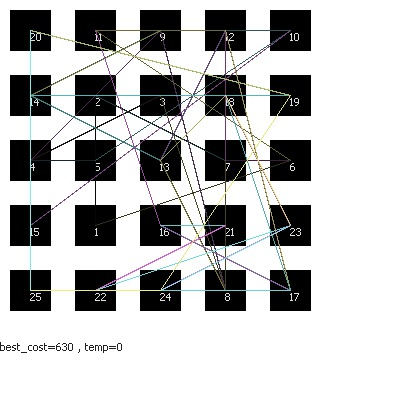
\includegraphics[scale=0.05]{image/state_000000.jpg}\\
\begin{center}
\textsc{Configuration de départ}\\
\end{center}
\end{minipage}}\\


\fbox{\begin{minipage}{0.9\textwidth}
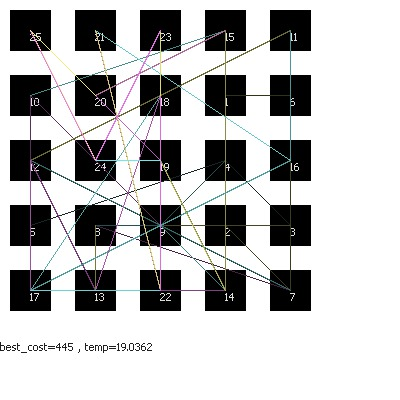
\includegraphics[scale=0.05]{image/state_000004.jpg}\\
\begin{center}
\textsc{Configuration avancée}\\
\end{center}
\end{minipage}}\\


\fbox{\begin{minipage}{0.9\textwidth}
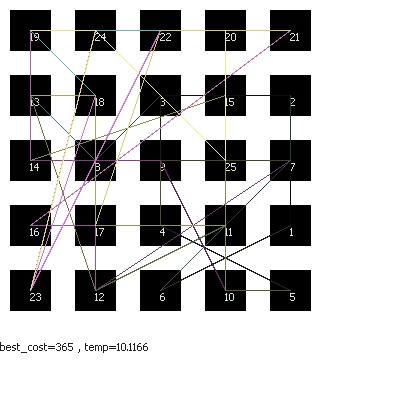
\includegraphics[scale=0.05]{image/state_000008.jpg}\\
\begin{center}
\textsc{Configuration plus avancée}\\
\end{center}
\end{minipage}}\\


\fbox{\begin{minipage}{0.9\textwidth}
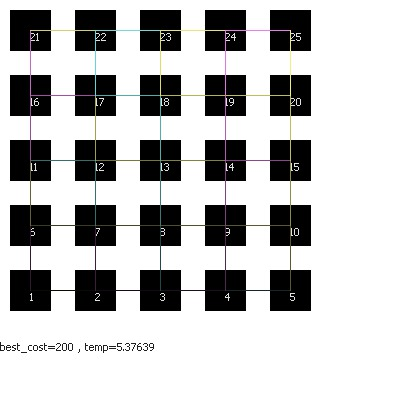
\includegraphics[scale=0.05]{image/state_000013.jpg}\\
\begin{center}
\textsc{Configuration de final}\\
\end{center}
\end{minipage}}\\


\section{Discussion sur le choix des paramètres}
La résolution d'un tel problème de référence, puisque l'on connaît à l'avance la solution, nous permet de mettre au point et de régler la méthode d'optimisation elle-même : cela permet d'étudier la sensibilité du recuit simulé par rapport au réglage de ses principaux paramètres.

Il convient d'abord d'identifier les différents paramètres du recuit simulé, à savoir :\\
- le $\tau 0$\\
- la décrémentation de la température\\
- le critère correspondant à l'équilibre thermodynamique\\
- la condition d'arrêt\\

En ce qui concerne la température, nous utilisons le $\tau 0$ pour dire ce que nous pensons de la solution initiale. Nous avons décidé de prendre un $\tau 0$ égale à 0.5 pour accepter environ une dégradation sur 2. Pour ce qui concerne la décrémentation de la température, nous multiplions la température par 0.9 en rapport avec ce que nous avons vu dans le cours et des résultats que nous avons pu avoir de notre coté. Il convient que la température de départ soit assez élevée dans la mesure où ainsi, on acceptera plus de dégradation en début et qu'on aura donc moins de chance de tomber dans un minimum local. Dans la même optique, la température ne doit pas être décrémenté trop brusquement, mais tout de même suffisante pour tendre vers une stabilisation du système sur le minimum global.

En ce qui concerne la condition d'arrêt, nous stoppons l'algorithme lorsque la température est inférieure à 0.000001 (chose qui n'arrive jamais), que l'on a atteint la configuration optimale de 200, ou que nous avons 3 palier de suite sans aucune acceptation puisque à ce moment on peut considérer qu'il n'y aura plus d'amélioration.

Les paramètres que nous avons choisis, nous permettent ainsi de trouver quasiment à coup sûr la solution du problème. Nous pourrions assouplir les paramètres choisis afin de faire moins d'itérations mais en pratique l'algorithme fonctionne très vite et de façon satisfaisante.

\newpage

\chapter{Cas discret avec la recherche tabou}
\minitoc
\section{Rappel du sujet}

Nous allons tout d’abord rappelé le sujet de l’exercice à résoudre, en ce qui concerne
le cas discret avec la recherche tabou.

Il s’agissait de résoudre un problème de placement de composants électroniques
en des sites prédéterminés. Il faut placer 25 blocs. Le seul mouvement autorisé est
la permutation de deux blocs. La fonction objectif, qu’il convient de minimiser, est
évaluée en sommant les longueurs en L (dites aussi « longueurs de Manhattan ») des
connexions. La distance entre deux blocs est égale à 5. Nous savons que pour les
configurations optimales, la fonction objectif est égale à 200, ce qui nous permettra
d’évaluer l’efficacité de notre méthode. Notons que les composants voisins sont définis dès le départ. Ainsi le composant numéro 8 doit être relié avec les composants
numéro 13, 3, 7 et 9. Les captures d’écran de notre application sont, à ce sujet, sans
doute plus claires qu’un long discours ; le lecteur perdu est donc invité à s’y référer.

Nous avons choisi d’implémenter la méthode de la recherche tabou qui semblait bien
adaptée pour résoudre ce problème.

\section{La recherche Tabou}
Nous n’allons pas détailler les différentes techniques rattachées à  cette méthode, car ce n’est pas le
propos de ce rapport. Nous allons, toutefois, récapituler très brièvement, les grands
traits caractéristiques de la recherche tabou.

La recherche tabou est une métaheuristique d'optimisation présentée par Fred Glover en 1986.
L'idée de la recherche tabou consiste, à partir d'une position donnée, à regarder les positions dans le voisinage et à choisir la position dans ce voisinage qui minimise la fonction objectif.
On peut noter que cette opération peut augmenter la valeur d'une fonction à minimiser : Si par exemple tous les points du voisinage ont une valeur plus élevée. C'est à partir de ce mécanisme que l'on sort d'un minimum local.

Le risque cependant est qu'à l'étape suivante, on retombe dans le minimum local auquel on vient d'échapper. C'est pourquoi il faut que l'heuristique ait de la mémoire : le mécanisme consiste à interdire de revenir sur les dernières positions explorées.C'est de là que vient le terme tabou.

Les positions déjà explorées sont conservées dans une file FIFO appelée  liste tabou  que l'on ajuste au besoin de l'heuristique. Cette file doit conserver des beaucoup de positions, ce qui peut  nécessiter la mise en mémoire d'une grande quantité d'informations. Cette difficulté peut être contournée gardant en mémoire que les mouvements précédents, associés à la valeur de la fonction à minimiser.

La méthode utilise une ou plusieurs mémoires  qui sont mises à jour
et exploitées au cours de la recherche.
Algorithme tabou de base : mémoire à court terme (liste taboue)
Algorithme tabou évolué : mémoire à court terme (liste tabou) et une mémoire à
long terme pour assurer l’intensification et/ou la diversification

L'idée de base de l'intensification vient qu on pourrait tenter d'approfondir (ou intensifier) des solutions qui semblaient prometteuses.

La diversification est pour eviter le problème de confinage. On fait en sorte de re diversifier les solutions pour explorer de nouveaux secteurs.

Voyons comment cela se traduit concrètement, en pratique, sur notre problème.

\begin{algorithm}
\caption{Calcul de la configuration optimale}
\begin{algorithmic}
\REQUIRE listetabou
\ENSURE configuration optimale
\WHILE{solution different de optimal}
\STATE Deplacement(listetabou)
\STATE Memorisation dans la liste tabou
\STATE Memorisation dans la memoire à long terme
\STATE Memroisation solution d'élite
\STATE compteur1++
\STATE compteur2++
\STATE test : methode: d'intensification
\STATE test : methode de diversification
\ENDWHILE
\end{algorithmic}
\end{algorithm}

\begin{algorithm}
\caption{Methode d'intensification}
\begin{algorithmic}
\REQUIRE x
\ENSURE 
\IF{stagnation || cycle1 == x}
\STATE search solution d'élite
\STATE retour à solution d'élite
\STATE mouvement différent de (liste bon placementdejaeffectuer)
\ENDIF
\STATE compteur1 = 0
\end{algorithmic}
\end{algorithm}

\begin{algorithm}
\caption{Methode de diversification par relance}
\begin{algorithmic}
\REQUIRE y
\ENSURE 
\IF{cycle2 == y}
\STATE Search memoire à long terme(element peu utilisé)
\STATE mouvement(element peu utilisé)
\ENDIF
\STATE compteur2 = 0
\end{algorithmic}
\end{algorithm}

\section{Réalisation}
\subsection{Choix techniques}
Nous avons choisi d'implémenter l'algorithme en C++, notamment dans un souci de performance d’exécution. On cherche en effet à obtenir la meilleure solution possible dans un délai de temps le plus court possible. 

\subsection{Implémentation}
 Nous allons brièvement aborder ici quelques points de l’algorithme qui peuvent poser problèmes.

Il nous a fallu développer une fonction pour calculer le coût d'une solution, puisque l'on cherche à minimiser ce coût qui représente la fonction objectif, et une fonction qui échange 2 pièces, puisque c'est cette transformation qui a été choisit.

Une fois que l'on a ces deux fonctions, on tire une configuration initiale aléatoirement et on applique l'algorithme.

La méthode de recherche tabou de base ne suffisant pas il a fallu adopter une recherche tabou evolué : c'est à dire doté d'une mémoire à long terme.On a doté la mémoire à long terme d'une technique de diversification et d 'une d'intensification.

On a choisi de memoriser les meilleurs solutions rencontrées au cours de la recherche (dite solutions d'élite) et on a choisi d'implementer la technique d'intensification suivante.
Lorsqu'il y a stagnation ou à partir d'un certain nombre de cycle on repart d'une solution d'élite
et on fixe les composants qui semblent intéressant c'est à dire faisant parti de plusieurs solutions d'élite.
Pour la méthode de diversification on a adopté pour une méthode  de diversification par relance :
on interrompt periodiquement la recherche et on construit une solution avec des attributs peu utilisés. 

 nous utilisons une des fonctions fournit par la STL qui en l’occurrence permet de générer des nombres aléatoires de manière uniforme.

\subsection{Résultats}
Les résultats obtenus sont satisfaisants. L'algorithme trouve dans la plupart des cas la meilleur solution. Mais Il a tendance a beaucoup changer de position avant de trouver la solution.


\section{Discussion sur le choix des paramètres}
La résolution d'un tel problème de référence dont on connaît à l'avance la solution, nous permet de mettre au point et de régler la méthode d'optimisation elle-même : cela permet d'étudier l'importance des principaux paramètres de la recherche tabou.

Il convient d'abord d'identifier les différents paramètres de la recherche tabou, à savoir :\\
- la taille de la liste tabou\\
- la condition d'arrêt\\
- Technique de diversification : nombre d'attribut\\

Pour la taille de la liste tabou, nous avons tester empiriquement la solution jusqu'a trouver un bon compromis pour trouver une solution satisfaisante. 
Pour le nombre d'attribut utilisé pour la relance on a pu voir qu'empiriquement une bonne solution etait de prendre 5 attributs.

Pour la condition d'arrêt, nous stoppons l'algorithme lorsque la durée de traitement est supérieur à un T = 1 heure(chose qui n'arrive jamais), que l'on a atteint la configuration optimale de 200.

Les paramètres que nous avons choisis, nous permettent ainsi de trouver quasiment à coup sûr la solution du problème.
\chapter{Conclusion générale}
Nous avons implémenté avec succès deux métaheuristiques pour l'optimisation difficile à savoir le recuit simulé et la recherche tabou pour répondre à un problème discret. Les deux méthodes se sont montrés très efficaces. Nous avons aussi pu réaliser l'importance des paramètres dans ces méthodes et la difficulté pratique de trouver les meilleurs paramètres selon les variations des problèmes qui se posent. On pourrait sans doute proposer des "metametaheuristiques" qui seraient capables d’utiliser une métaheuristique et de trouver
les meilleurs paramètres de cette métaheuristique selon le problème posé. Pourquoi
ne pas imaginer par exemple une application utilisant un essaim particulaire dont les
meilleurs paramètres pour une fonction donnée seraient trouvés par recuit simulé ?
\end{document}
